


\begin{frame}{Before we start...}

   \begin{block}{Goal of this Workshop}
    \begin{itemize}
     \item {\Huge \textbf{\color{red} You}} are here to learn new things about HPC
    \end{itemize}
   \end{block}

   \vspace*{1cm}
   \begin{block}{Ask Questions}
    \begin{itemize}
     \item Tell me if you do not understand
     \item Ask for further details
     \item Don't be shy
    \end{itemize}
   \end{block}

\end{frame}




\begin{frame}{Table of Contents}
   \begin{block}{$p$-Bratu Equation} \end{block}
   \begin{block}{Distributed Arrays} \end{block}
   \begin{block}{Nonlinear Solvers} \end{block}
   \begin{block}{Matrices, Linear Solvers} \end{block}
   \begin{block}{Preconditioners} \end{block}
\end{frame}


%%%%%% General PETSc information %%%%%%%%%%

%
% Why Libraries?
%   - Reinvent the wheel again and again?
%   - Same procedure common for non-software (Theorems, engineering, etc.)
%   - Specialization and settlement of approaches over time (OS, Hardware, etc.)
%   





%
%%%%% p-Bratu
%
\section{p-Bratu Equation}
\begin{frame}{PETSc}
   \begin{center} \Large \textbf{$p$-Bratu Equation} \end{center}
\end{frame}





\begin{frame}{The $\mathfrak{p}$-Bratu Equation}

  \begin{block}{The ``Hello World of PDEs''}
  \begin{itemize}
   \item Poisson's Equation
    \begin{equation*}
      -\nabla \cdot \bigl(\nabla u \bigr) = f,
    \end{equation*}
   \item Leads to symmetric, positive definite system matrices
   \item Commonly used in numerical analysis (corner effects, etc.)
  \end{itemize}
  \end{block}

  \begin{block}{More General Form}
  \begin{itemize}
   \item With diffusivity tensor $\eta$:
    \begin{equation*}
      -\nabla \cdot \bigl( \eta \nabla u \bigr) = f,
    \end{equation*}
   \item Typically: $\eta > \delta > 0$
   \item $\eta$ can be discontinous (material boundaries)
   \item Reduced regularity of solution
  \end{itemize}
  \end{block}
  
\end{frame}


\begin{frame}{The $\mathfrak{p}$-Bratu Equation}

  \begin{block}{Additional Volume Term}
  \begin{itemize}
   \item Consider
    \begin{equation*}
      -\nabla \cdot \bigl(\eta \nabla u \bigr) - \lambda e^u - f = 0 \ ,
    \end{equation*}
   \item Canonical nonlinear form
   \item $e^u$ has ``wrong sign'': turning point at $\lambda_{\text{crit}}$
  \end{itemize}
  \end{block}

  \begin{block}{Another Tweak}
  \begin{itemize}
   \item Diffusivity tensor $\eta$ depends on $u$, e.g.:
    \begin{equation*}
      \eta = \frac{1}{2} \vert \nabla u \vert^2,
    \end{equation*}
   \item Singular or degenerate when $\nabla u = 0$.
  \end{itemize}
  \end{block}
  
\end{frame}


% \section{$\pfrak$-Bratu}
\begin{frame}{The $\mathfrak{p}$-Bratu Equation}

  \begin{block}{$\mathfrak{p}$-Bratu Equation}
  \begin{itemize}
  \item 2-dimensional model problem
    \begin{equation*}
      -\nabla \cdot \bigl(\vert\nabla u\vert^{\mathfrak{p}-2} \nabla u \bigr) - \lambda e^u - f = 0, \qquad 1 \le \mathfrak{p} \le \infty, \quad \lambda < \lambda_{\text{crit}}(\mathfrak{p})
    \end{equation*}
    Singular or degenerate when $\nabla u = 0$, turning point at $\lambda_{\text{crit}}$.
  \end{itemize}
  \end{block}
  
  \begin{block}{Regularized Variant}
  \begin{itemize}
  \item Remove singularity of $\eta$ using a parameter $\varepsilon$:
    \begin{gather*}
      -\nabla \cdot (\eta \nabla u) - \lambda e^u - f = 0 \\
      \eta(\gamma) = (\epsilon^2 + \gamma)^{\frac{\mathfrak{p}-2}{2}} \qquad \gamma(u) = \frac{1}{2} \vert\nabla u\vert^2
    \end{gather*}
  \item       Physical interpretation: diffusivity tensor flattened in direction $\nabla u$
  \end{itemize}
  \end{block}
\end{frame}








%
%%%%% Distributed Arrays
%
\section{Distributed Arrays}
\begin{frame}{PETSc}
   \begin{center} \Large \textbf{Distributed Arrays} \end{center}
\end{frame}

\begin{frame}[fragile]{Distributed Array}

  \begin{block}{Interface for topologically structured grids}
  \end{block}

  \begin{block}{Defines (topological part of) a finite-dimensional function space}
    \begin{itemize} 
      \item Get an element from this space: \lstinline|DMCreateGlobalVector()| 
    \end{itemize}
  \end{block}

  \begin{block}{Provides parallel layout}
  \end{block}

  \begin{block}{Refinement and coarsening}
    \begin{itemize}
      \item \lstinline|DMRefineHierarchy()| 
    \end{itemize}
  \end{block}

  \begin{block}{Ghost value coherence}
    \begin{itemize}
       \item \lstinline|DMGlobalToLocalBegin()|
     \end{itemize}
  \end{block}

  \begin{block}{Matrix preallocation}
       \begin{itemize}
         \item \lstinline|DMCreateMatrix()| (formerly \lstinline|DMGetMatrix()|) 
       \end{itemize}
  \end{block}
\end{frame}

\begin{frame}
\frametitle{Ghost Values}

\begin{block}{To evaluate a local function $f(x)$, each process requires}
\begin{itemize}
  \item its local portion of the vector $x$
  \item its {\color{cyan}ghost values}, bordering portions of $x$ owned by neighboring processes
\end{itemize}
\end{block}

\begin{center}
\includegraphics[width=4in]{figures/GhostValues}
\end{center}

\end{frame}

\input{slides/DA/GlobalNumberings.tex}
\begin{frame}{DMDA Global vs. Local Numbering}

\begin{itemize}
  \item {\bf Global}: Each vertex has a unique id, belongs on a unique process

  \item {\bf Local}: Numbering includes vertices from neighboring processes
  \begin{itemize}
    \item These are called {\color{cyan}ghost} vertices
  \end{itemize}
\end{itemize}

\begin{center}
\begin{tabular}{cc}
\begin{tabular}{c}
\begin{tabular}{|ccc|cc|}
\hline
\multicolumn{3}{|c|}{Proc 2} & \multicolumn{2}{c|}{Proc 3} \\
\hline
 X &  X &  X &  X &  X \\
 X &  X &  X &  X &  X \\
{\color{cyan}12} & {\color{cyan}13} & {\color{cyan}14} & {\color{cyan}15} &  X \\
\hline
 8 &  9 & 10 & {\color{cyan}11} &  X \\
 4 &  5 &  6 & {\color{cyan}7} &  X \\
 0 &  1 &  2 & {\color{cyan}3} &  X \\
\hline
\multicolumn{3}{|c|}{Proc 0} & \multicolumn{2}{c|}{Proc 1} \\
\hline
\end{tabular} \\
Local numbering
\end{tabular}
& 
\begin{tabular}{c}
\begin{tabular}{|ccc|cc|}
\hline
\multicolumn{3}{|c|}{Proc 2} & \multicolumn{2}{c|}{Proc 3} \\
\hline
21 & 22 & 23 & 28 & 29 \\
18 & 19 & 20 & 26 & 27 \\
15 & 16 & 17 & 24 & 25 \\
\hline
 6 &  7 &  8 & 13 & 14 \\
 3 &  4 &  5 & 11 & 12 \\
 0 &  1 &  2 &  9 & 10 \\
\hline
\multicolumn{3}{|c|}{Proc 0} & \multicolumn{2}{c|}{Proc 1} \\
\hline
\end{tabular}\\
Global numbering
\end{tabular}
\end{tabular}
\end{center}
\end{frame}




\begin{frame}[fragile]{PETSc Vectors}

 \begin{block}{Parallel Vector Layout}
   \begin{center}
     \includegraphics[width=0.75\textwidth]{figures/vectors} \\[2em]
   \end{center}
\begin{lstlisting}
  VecCreate(PETSC_COMM_WORLD, &x);
  VecSetSizes(x, PETSC_DECIDE, N);
  VecSetFromOptions(x);
\end{lstlisting}
  \vspace*{2.3cm}
 \end{block}

\end{frame}

\begin{frame}[fragile]{PETSc Vectors}

 \begin{block}{Vector Gather and Scatter}
   \begin{center}
     \includegraphics[width=0.75\textwidth]{figures/vectors-scatter} \\[1em]
\begin{lstlisting}
  // y[iy[i]] = x[ix[i]]
  VecScatterCreate(...);
  VecScatterBegin(...);
  VecScatterEnd(...);
\end{lstlisting}
   \end{center}
 \end{block}

\end{frame}

%%%%%%%%%% 


\begin{frame}[fragile]{PETSc Vectors}

 \begin{block}{Vector Reductions}
   \begin{center}
     \includegraphics[width=0.75\textwidth]{figures/vectors-reduce} \\[1.2em]
\begin{lstlisting}
  VecNorm(...);
  VecDot(...);
  VecMax(...);
  ...
\end{lstlisting}
   \end{center}
 \end{block}

\end{frame}


%%%%%%%%%% 

\begin{frame}[fragile]{PETSc Vectors}

 \begin{block}{Local (Sequential) Operations}
  \begin{itemize}
   \item Executed by an arbitrary subset of MPI ranks
   \item Usually involve \lstinline|VecGetArray()/VecRestoreArray()|
  \end{itemize}
 \end{block}

 %\pause
 
 \begin{block}{Collective Operations}
  \begin{itemize}
   \item Must be executed by all processes in the MPI communicator
   \item Involve MPI operations (scatter, gather, reduce, etc.)
  \end{itemize}
 \end{block}

\end{frame}

\begin{frame}{Updating Ghosts}

\begin{block}{Two-step Process for Updating Ghosts}
 \begin{itemize}
  \item enables overlapping computation and communication
 \end{itemize}
\end{block}
 

\begin{block}{\lstinline|DMGlobalToLocalBegin(dm, gvec, mode, lvec)|}
  \begin{itemize}
    \item \lstinline|gvec| provides the data 
    \item \lstinline|mode| is either \lstinline|INSERT_VALUES| or \lstinline|ADD_VALUES|
    \item \lstinline|lvec| holds the local and ghost values
  \end{itemize}
\end{block}

\begin{block}{\lstinline|DMGlobalToLocalEnd(dm, gvec, mode, lvec)|}
  \begin{itemize}
    \item Finishes the communication
  \end{itemize}
\end{block}

\medskip

\begin{block}{Reverse Process}
  \begin{itemize}
   \item Via \lstinline|DMLocalToGlobalBegin()| and \lstinline|DMLocalToGlobalEnd()|.
  \end{itemize}
\end{block}
 
\end{frame}

\begin{frame}
\frametitle{DMDA Stencils}

\begin{block}{Available Stencils}
%  \begin{itemize}
%   \item {\color{blue}box} stencil
%   \item {\color{blue}star} stencil
%  \end{itemize}
\end{block}

\begin{center}
\includegraphics[width=0.95\textwidth]{figures/DA/Stencils}
\end{center}
\end{frame}

\begin{frame}[fragile]
\frametitle{Creating a DMDA}

{\small \lstinline|DMDACreate2d(comm, xbdy, ybdy, type, M, N, m, n|, \\
\qquad\qquad\qquad \qquad  \lstinline|dof, s, lm[], ln[], DA *da)|}

\begin{block}{\lstinline|xbdy,ybdy|: Specifies periodicity or ghost cells}
  \vspace*{-0.2cm}
  \begin{itemize}
    \item \lstinline|DM_BOUNDARY_NONE|, \lstinline|DM_BOUNDARY_GHOSTED|, \lstinline|DM_BOUNDARY_MIRROR|, \lstinline|DM_BOUNDARY_PERIODIC|
  \end{itemize}
\end{block}

\vspace*{-0.3cm}
\begin{block}{\lstinline|type|}
  \vspace*{-0.2cm}
  \begin{itemize}
    \item Specifies stencil: \lstinline|DMDA_STENCIL_BOX| or \lstinline|DMDA_STENCIL_STAR|
  \end{itemize}
\end{block}

\vspace*{-0.3cm}
\begin{block}{\lstinline|M,N|}
  \vspace*{-0.2cm}
  \begin{itemize}
    \item Number of grid points in x/y-direction
  \end{itemize}
\end{block}

\vspace*{-0.3cm}
\begin{block}{\lstinline|m,n|}
  \vspace*{-0.2cm}
  \begin{itemize}
    \item Number of processes in x/y-direction
  \end{itemize}
\end{block}

\vspace*{-0.3cm}
\begin{block}{\lstinline|dof|}
  \vspace*{-0.2cm}
  \begin{itemize}
    \item Degrees of freedom per node
  \end{itemize}
\end{block}

\vspace*{-0.3cm}
\begin{block}{\lstinline|s|}
  \vspace*{-0.2cm}
  \begin{itemize}
    \item The stencil width
  \end{itemize}
\end{block}

\vspace*{-0.3cm}
\begin{block}{\lstinline|lm,ln|}
  \vspace*{-0.2cm}
  \begin{itemize}
    \item Alternative array of local sizes
    \item Use \lstinline|NULL| for the default
  \end{itemize}
\end{block}

\end{frame}

\begin{frame}[fragile]{Working with the Local Form}

\begin{block}{Wouldn't it be nice if we could just write our code for the natural numbering?}
 
 \only<1>{
\begin{center}
\begin{tabular}{cc}
\begin{tabular}{c}
\begin{tabular}{|ccc|cc|}
\hline
\multicolumn{3}{|c|}{Proc 2} & \multicolumn{2}{c|}{Proc 3} \\
\hline
25 & 26 & 27 & 28 & 29 \\
20 & 21 & 22 & 23 & 24 \\
15 & 16 & 17 & 18 & 19 \\
\hline
10 & 11 & 12 & 13 & 14 \\
 5 &  6 &  7 &  8 &  9 \\
 0 &  1 &  2 &  3 &  4 \\
\hline
\multicolumn{3}{|c|}{Proc 0} & \multicolumn{2}{c|}{Proc 1} \\
\hline
\end{tabular} \\
Natural numbering
\end{tabular}
& 
\begin{tabular}{c}
\begin{tabular}{|ccc|cc|}
\hline
\multicolumn{3}{|c|}{Proc 2} & \multicolumn{2}{c|}{Proc 3} \\
\hline
21 & 22 & 23 & 28 & 29 \\
18 & 19 & 20 & 26 & 27 \\
15 & 16 & 17 & 24 & 25 \\
\hline
 6 &  7 &  8 & 13 & 14 \\
 3 &  4 &  5 & 11 & 12 \\
 0 &  1 &  2 &  9 & 10 \\
\hline
\multicolumn{3}{|c|}{Proc 0} & \multicolumn{2}{c|}{Proc 1} \\
\hline
\end{tabular}\\
PETSc numbering
\end{tabular}
\end{tabular}
\end{center}
\vspace*{1cm}
    }
    
    
 \only<2>{
  \begin{itemize}
  \item Yes, that's what \lstinline|DMDAVecGetArray()| is for.
  \end{itemize}
  }
  
  \end{block}
  
  \only<2>{
 \begin{block}{DMDA offers \emph{local} callback functions}
    \begin{itemize}
      \item \lstinline|FormFunctionLocal()|, set by \lstinline|DMDASetLocalFunction()|
      \item \lstinline|FormJacobianLocal()|, set by \lstinline|DMDASetLocalJacobian()|
    \end{itemize}
 \end{block}

 
 \begin{block}{Evaluating the nonlinear residual $F(x)$}
    \begin{itemize}
      \item Each process evaluates the local residual
      \item PETSc assembles the global residual automatically
        \begin{itemize}
        \item Uses \lstinline|DMLocalToGlobal()| method
        \end{itemize}
    \end{itemize}
 \end{block}
 }

\end{frame}

\begin{frame}[fragile]{Thinking of Extensions}

\begin{block}{Multiple Unknowns per Grid Node}
  \begin{itemize}
   \item Example 1: Displacements $u_x$, $u_y$
   \item Example 2: Velocity components, Pressure
   \item Typical in a multiphysics setting
  \end{itemize}
\end{block}

\begin{block}{Multiple Unknowns in a Distributed Setting}
  \begin{itemize}
   \item Robust abstract concepts important
   \item Lots of bookkeeping
   \item All done by PETSc
  \end{itemize}

\end{block}

\end{frame}


\begin{frame}[fragile]{Thinking of Extensions}

\begin{center}
 \includegraphics[width=\textwidth]{figures/localspaces}
\end{center}


\end{frame}

\begin{frame}[fragile]
\frametitle{DA Local Function}

\begin{block}{User-provided Function for Nonlinear Residual in 2D}
\begin{lstlisting}
  PetscErrorCode (*lfunc)(DMDALocalInfo *info,
                          Field **x, Field **r,
                          void *ctx)
\end{lstlisting}

\begin{tabular}{lp{8.3cm}}
  \lstinline|info| & All layout and numbering information \\
  \lstinline|x|    & The current solution \newline
     \emph{ Notice that it is a multidimensional array} \\
  \lstinline|r|    & The residual \\
  \lstinline|ctx|  & The user context passed to \lstinline|DMSetApplicationContext()| or to SNES \\
\end{tabular}


\bigskip

The local DMDA function is activated by calling
\begin{itemize}
 \item \lstinline|SNESSetDM(snes,dm)|
 \item \lstinline|SNESSetFunction(snes, r, SNESDAFormFunction, ctx)|
\end{itemize}
\end{block}
\end{frame}




%%
%% Discretizations
%% 

% Finite Differences
% Finite Volumes
% Finite Elements
% Other approaches

\begin{frame}{Discretization}
 
 \begin{block}{Mapping PDEs to a (un)structured Grid}
   \begin{itemize}
    \item Can be arbitrarily complex (mathematically)
    \item Neverending area of research
   \end{itemize}
 \end{block}
 
 \begin{block}{Popular Discretization Schemes}
   \begin{itemize}
    \item Finite Difference Method
    \item Finite Volume Method
    \item Finite Element Method
   \end{itemize}
 \end{block}
 
\end{frame}

%%%%%%%%%%%%%%%%%%%%%%%

\begin{frame}{Finite Difference Methods}
 
 \begin{block}{Finite Difference Methods: $u'$}
   \begin{itemize}
    \item Consider 1d-grid
    \item Replace $u' \approx \frac{u[i+1] - u[i]}{h}$
    \item or $u' \approx \frac{u[i] - u[i-1]}{h}$
    \item or $u' \approx \frac{u[i+1] - u[i-1]}{2h}$
   \end{itemize}
 \end{block}
 
 %\vspace*{1cm}
 \begin{block}{Finite Difference Methods: $u''$}
   \begin{itemize}
    \item Naive: $u'' \approx \frac{u'[i+1] - u'[i-1]}{2h} \approx \frac{u[i+2] - 2u[i] + u[i-2]}{4h^2}$
    \item Use 'virtual' grid nodes $u'[i+0.5]$, $u'[i-0.5]$ to obtain
      \begin{align*}
        u''(x_i) \approx \frac{u[i+1] - 2u[i] + u[i-1]}{h^2}
      \end{align*}
   \end{itemize}
 \end{block}
 
 %\vspace*{-7cm}
 %\begin{flushright}
 % \includegraphics[width=0.55\textwidth]{figures/fd_stencil}
 %\end{flushright}
 %\vspace*{4cm}

 
\end{frame}



%%%%%%%%%%%%%%%%%%%%%%%

\begin{frame}{Finite Volume Methods}
 
 \begin{block}{Finite Volume Methods}
   \begin{itemize}
    \item Suitable for unstructured grids
    \item Popular for conservation laws
    \item Integrate PDE over box, apply Gauss' theorem
    \item On regular grid: (Almost) same expression as finite differences
   \end{itemize}
 \end{block}
 
 %\begin{center}
 % \includegraphics[width=0.4\textwidth]{figures/finite-volume}
 %\end{center}
 
\end{frame}





%%%%%%%%%%%%%%%%%%%%%%%

\begin{frame}{Finite Element Methods}
 
 \begin{block}{Finite Element Methods}
   \begin{itemize}
    \item Ansatz: $u \approx \sum_i u_i \varphi_i$
    \item $\varphi_i$ piecewise polynomials of degree $p$
    \item Solve for $u_i$
    \item Adaptivity: in $h$ and/or $p$ possible
    \item Rich mathematical theory
   \end{itemize}
 \end{block}
 
 %\begin{center}
 % \includegraphics[width=0.5\textwidth]{figures/finite_element_method}
 %\end{center}
 
\end{frame}




\input{slides/DA/BratuResidual.tex}

%% Go through first code example


%
% Nonlinear Solvers
%
\section{Nonlinear Solvers}
\begin{frame}{PETSc}
   \begin{center} \Large \textbf{Nonlinear Solvers} \end{center}
\end{frame}


\begin{frame}{Newton iteration: Workhorse of SNES}
  \begin{flushright}
    \includegraphics[width=0.25\textwidth]{figures/Newton}
  \end{flushright}
  \vspace*{-4cm}
  \begin{block}{Standard form of a nonlinear system}
    \[ \hspace*{-1cm} -\nabla \cdot \bigl(\vert\nabla u\vert^{\mathfrak{p}-2} \nabla u \bigr) - \lambda e^u = F(u) = 0 \]
  \end{block}
  
  \begin{block}{Iteration}
    \vspace*{-0.5cm}
    \begin{align*}
      \text{Solve:} & \qquad J(u) w = -F(u) \\
      \text{Update:} & \qquad u^+ \gets u + w
    \end{align*}
    \begin{itemize}
    \item Quadratically convergent near a root: $|u^{n+1}-u^*| \in \mathcal{O} \Big(|u^n-u^*|^2\Big)$
    \item Picard is the same operation with a different $J(u)$
    \end{itemize}
  \end{block}
  
  \begin{block}{Jacobian Matrix for $\mathfrak{p}$-Bratu Equation}
    \vspace*{-0.5cm}
        \begin{gather*}
         J(u) w \sim -\nabla \bigl[ (\eta {\mathbf{1}} + \eta' \nabla u \otimes \nabla u) \nabla w \bigr] - \lambda e^u w \\
          \eta' = \frac{\mathfrak{p}-2}{2} \eta / (\epsilon^2 + \gamma)
        \end{gather*}
  \end{block}
\end{frame}


\begin{frame}{SNES}
  
  \begin{block}{Scalable Nonlinear Equation Solvers}
    \begin{itemize}
     \item Newton solvers: Line Search, Thrust Region
     \item Inexact Newton-methods: Newton-Krylov
     \item Matrix-Free Methods: With iterative linear solvers
    \end{itemize}
  \end{block}
  
  \begin{block}{How to get the Jacobian Matrix?}
    \begin{itemize}
     \item Implement it by hand
     \item Let PETSc finite-difference it
     \item Use Automatic Differentiation software
    \end{itemize}
  \end{block}
\end{frame}

\input{slides/SNES/NonlinearSolversList.tex}

%\begin{frame}[fragile]
\frametitle{Flow Control for a PETSc Application}

\begin{center}
\includegraphics[width=4.0in]{figures/FlowControl}
\end{center}
\end{frame}

\begin{frame}[fragile]
\frametitle{SNES Paradigm}

\begin{block}{SNES Interface based upon Callback Functions}
\begin{itemize}
  \item \lstinline|FormFunction()|, set by \lstinline|SNESSetFunction()|
  \item \lstinline|FormJacobian()|, set by \lstinline|SNESSetJacobian()|
\end{itemize}
\end{block}
%\bigskip

 \begin{block}{Evaluating the nonlinear residual $F(x)$}
\begin{itemize}
  \item Solver calls the \textbf{user's} function

  \medskip

  \item User function gets application state through the \lstinline|ctx| variable
\end{itemize}
 \end{block}

   \begin{center}
    \color{red} PETSc \emph{never} sees application data
  \end{center}

\end{frame}

\begin{frame}[fragile]{SNES Function}

\begin{align*}
 F(u) = 0
\end{align*}

The user provided function which calculates the nonlinear residual has signature
\begin{lstlisting}
  PetscErrorCode (*func)(SNES snes,
                         Vec x,Vec r,
                         void *ctx)
\end{lstlisting}

\begin{itemize}
  \item \lstinline|x| - The current solution
  \item \lstinline|r| - The residual
  \item \lstinline|ctx| -  The user context passed to \lstinline|SNESSetFunction()|
  \begin{itemize}
    \item Use this to pass application information, e.g.~physical constants
  \end{itemize}
\end{itemize}

\end{frame}

\begin{frame}[fragile]{SNES Jacobian}

\begin{block}{User-provided function calculating the Jacobian Matrix}
\begin{lstlisting}
PetscErrorCode (*func)(SNES snes,Vec x,Mat *J,Mat *M,
                       MatStructure *flag,void *ctx)
\end{lstlisting}

\begin{itemize}
  \item \lstinline|x| - The current solution
  \item \lstinline|J| - The Jacobian
  \item \lstinline|M| -  The Jacobian preconditioning matrix (possibly J itself)
  \item \lstinline|ctx| - The user context passed to \lstinline|SNESSetFunction()|
  \begin{itemize}
    \item Use this to pass application information, e.g. physical constants
  \end{itemize}

  \item Possible \lstinline|MatStructure| values are:
  \begin{itemize}
    \item \lstinline|SAME_NONZERO_PATTERN|
    \item \lstinline|DIFFERENT_NONZERO_PATTERN|
  \end{itemize}
\end{itemize}
\end{block}

\begin{block}{Alternatives}
\begin{itemize}
  \item a builtin sparse finite difference approximation (``coloring'')
  \item automatic differentiation (ADIC/ADIFOR)
\end{itemize}
\end{block}

\end{frame}

\begin{frame}[fragile]{Finite Difference Jacobians}

\begin{block}{PETSc can compute and explicitly store a Jacobian}
 
 \begin{itemize}
  \item Dense
    \begin{itemize}
    \item Activated by \lstinline|-snes_fd|
    \item Computed by \lstinline|SNESDefaultComputeJacobian()|
    \end{itemize}
  \item Sparse via colorings
    \begin{itemize}
    \item Coloring is created by \lstinline|MatFDColoringCreate()|
    \item Computed by \lstinline|SNESDefaultComputeJacobianColor()|
    \end{itemize}
  \end{itemize}
  
\end{block}

  \begin{block}{Also Matrix-free Newton-Krylov via 1st-order FD possible}
  \begin{itemize}
  \item Activated by \lstinline|-snes_mf| without preconditioning
  \item Activated by \lstinline|-snes_mf_operator| with user-defined preconditioning
    \begin{itemize}
    \item Uses preconditioning matrix from \lstinline|SNESSetJacobian()|
    \end{itemize}
  \end{itemize}
  \end{block}

\end{frame}


\begin{frame}[fragile]{DMDA and SNES}
 
  \begin{block}{Fusing Distributed Arrays and Nonlinear Solvers}
   \begin{itemize}
    \item Make DM known to SNES solver
      \begin{lstlisting}
 SNESSetDM(snes,dm);
      \end{lstlisting}

    \item Attach residual evaluation routine
      \begin{lstlisting}
 DMDASNESSetFunctionLocal(dm,INSERT_VALUES,
        (DMDASNESFunction)FormFunctionLocal,
                          &user);
      \end{lstlisting}
   \end{itemize}
  \end{block}

  \begin{block}{Ready to Roll}
   \begin{itemize}
    \item First solver implementation completed
    \item Uses finite-differencing to obtain Jacobian Matrix
    \item Rather slow, but scalable!
   \end{itemize}
  \end{block}

 
\end{frame}







%
% Matrices (preparing for Linear Solvers)
%

\section{Matrices in PETSc}
\begin{frame}{PETSc}
   \begin{center} \Large \textbf{Matrices} \end{center}
\end{frame}


\begin{frame}[fragile]{PETSc Application Integration}

\begin{block}{Sparse Matrices}
\begin{itemize}
  \item \textbf{The} important data type when solving PDEs
  \item Two main phases: 
    \begin{itemize}
     \item Filling with entries (assembly)
     \item Application of its action (e.g.~SpMV)
    \end{itemize}
\end{itemize}
\end{block}
\begin{center}
%\includegraphics[width=2in]{figures/Mat/serialSparseMatrix_bcsstk32}
\includegraphics[width=.5\textwidth]{figures/EllipRCMSquare}
\end{center}
\end{frame}



\begin{frame}[fragile]{Matrix Memory Preallocation}
 \begin{block}{PETSc sparse matrices are dynamic data structures}
  \begin{itemize} \vspace*{-0.2cm}
    \item can add additional nonzeros freely
  \end{itemize}
 \end{block}  \vspace*{-0.2cm}

 %\pause
 \begin{block}{Dynamically adding many nonzeros}
  \begin{itemize} \vspace*{-0.2cm}
    \item requires additional memory allocations
    \item requires copies
    \item can kill performance
  \end{itemize}
 \end{block} \vspace*{-0.2cm}

 %\pause
 \begin{block}{Memory preallocation provides}
  \begin{itemize} \vspace*{-0.2cm}
    \item the freedom of dynamic data structures
    \item good performance
  \end{itemize}
 \end{block} \vspace*{-0.2cm}

 %\pause
 \begin{block}{Easiest solution is to replicate the assembly code}
  \begin{itemize} \vspace*{-0.2cm}
    \item Remove computation, but preserve the indexing code
    \item Store set of columns for each row
  \end{itemize}
 \end{block} \vspace*{-0.2cm}

 %\pause
 \begin{block}{Call preallocation routines for all datatypes}
  \begin{itemize} \vspace*{-0.2cm}
    \item \lstinline|MatSeqAIJSetPreallocation()|
    \item \lstinline|MatMPIBAIJSetPreallocation()|
    \item Only the relevant data will be used
  \end{itemize}
\end{block}
\end{frame}




\begin{frame}[fragile]{PETSc Application Integration}

\begin{block}{Sequential Sparse Matrices}
\lstinline|MatSeqAIJSetPreallocation(Mat A, int nz, int nnz[])|
\hbox{\qquad
\vbox{
\begin{itemize}
  \item[nz:] expected number of nonzeros in any row
  \item[nnz(i):] expected number of nonzeros in row i
\end{itemize}
}
}
\end{block}
\begin{center}
%\includegraphics[width=2in]{figures/Mat/serialSparseMatrix_bcsstk32}
\includegraphics[width=.5\textwidth]{figures/EllipRCMSquare}
\end{center}
\end{frame}

\begin{frame}[fragile]{PETSc Application Integration}

\begin{block}{Parallel Sparse Matrix}
\begin{itemize}
  \item Each process locally owns a submatrix of contiguous global rows
  \item Each submatrix consists of diagonal and off-diagonal parts
\end{itemize}

\begin{center}
\includegraphics[width=3.in]{figures/Mat/parallelSparseMatrix}
\end{center}

\begin{itemize}
  \item \lstinline|MatGetOwnershipRange(Mat A,int *start,int *end)|
  \begin{itemize}
    \item \lstinline|start|: first locally owned row of global matrix
    \item \lstinline|end-1|: last locally owned row of global matrix
  \end{itemize}
\end{itemize}
\end{block}
\end{frame}


\begin{frame}[fragile]{PETSc Application Integration}

\begin{center}
\includegraphics[width=3.in]{figures/Mat/parallelSparseMatrix}
\end{center}

\begin{center}
\begin{tabular}{cc}
\begin{tabular}{c}
\begin{tabular}{|ccc|cc|}
\hline
\multicolumn{3}{|c|}{Proc 2} & \multicolumn{2}{c|}{Proc 3} \\
\hline
25 & 26 & 27 & 28 & 29 \\
20 & 21 & 22 & 23 & 24 \\
15 & 16 & 17 & 18 & 19 \\
\hline
10 & 11 & 12 & 13 & 14 \\
 5 &  6 &  7 &  8 &  9 \\
 0 &  1 &  2 &  3 &  4 \\
\hline
\multicolumn{3}{|c|}{Proc 0} & \multicolumn{2}{c|}{Proc 1} \\
\hline
\end{tabular} \\
Natural numbering
\end{tabular}
& 
\begin{tabular}{c}
\begin{tabular}{|ccc|cc|}
\hline
\multicolumn{3}{|c|}{Proc 2} & \multicolumn{2}{c|}{Proc 3} \\
\hline
21 & 22 & 23 & 28 & 29 \\
18 & 19 & 20 & 26 & 27 \\
15 & 16 & 17 & 24 & 25 \\
\hline
 6 &  7 &  8 & 13 & 14 \\
 3 &  4 &  5 & 11 & 12 \\
 0 &  1 &  2 &  9 & 10 \\
\hline
\multicolumn{3}{|c|}{Proc 0} & \multicolumn{2}{c|}{Proc 1} \\
\hline
\end{tabular}\\
PETSc numbering
\end{tabular}
\end{tabular}
\end{center}

\end{frame}








\begin{frame}[fragile]{PETSc Application Integration}

\begin{block}{Parallel Sparse Matrix}
\vspace{0.5cm}
\hbox{ \quad \vbox{
\begin{lstlisting}
 MatMPIAIJSetPreallocation(Mat A, int dnz, int dnnz[],
                                  int onz, int onnz[]
\end{lstlisting}

\begin{itemize}
  \item[dnz:] expected number of nonzeros in any row in the diagonal block
  \item[dnnz(i):] expected number of nonzeros in row i in the diagonal block
  \item[onz:] expected number of nonzeros in any row in the offdiagonal portion
  \item[onnz(i):] expected number of nonzeros in row i in the offdiagonal portion
\end{itemize}
}}
\end{block}
\end{frame}

\begin{frame}[fragile]{PETSc Application Integration}

\begin{block}{Verifying Preallocation}
\begin{itemize}
  \item Use runtime options 
    \begin{itemize}
      \item \lstinline|-mat_new_nonzero_location_err| 
      \item \lstinline|-mat_new_nonzero_allocation_err|
    \end{itemize}
    
  \item Use runtime option
    \begin{itemize} \item \lstinline|-info| \end{itemize}
  \item Output: \\
\end{itemize}

\end{block}
\begin{lstlisting}[basicstyle=\scriptsize]
[proc #] Matrix size: %d X %d; storage space: %d unneeded, %d used
[proc #] Number of mallocs during MatSetValues( )  is %d
\end{lstlisting}

\begin{center}
\includegraphics[width=4.in]{figures/logInfoOutput}
\end{center}
\end{frame}

\begin{frame}[fragile]{Block and Symmetric Formats}
  \begin{block}{BAIJ}
    \begin{itemize}
    \item Like AIJ, but uses static block size
    \item Preallocation is like AIJ, but just one index per block
    \end{itemize}
  \end{block}
  
  %\pause
  \begin{block}{SBAIJ}
    \begin{itemize}
    \item Only stores upper triangular part
    \item Preallocation needs number of nonzeros in upper triangular \\
      parts of on- and off-diagonal blocks
    \end{itemize}
  \end{block}
    
  %\pause
  \begin{block}{MatSetValuesBlocked()}
    \begin{itemize}
    \item Better performance with blocked formats
    \item Also works with scalar formats, if \lstinline|MatSetBlockSize()| was called
    \item Variants \lstinline|MatSetValuesBlockedLocal()|, \lstinline|MatSetValuesBlockedStencil()|
    \item Change matrix format at runtime, don't need to touch assembly code
    \end{itemize}
  \end{block}
\end{frame}

\input{slides/PETSc/Integration/MisguidedMatrixAssembly.tex}
\begin{frame}[fragile]{A Better Way to Set the Elements of a Matrix}

\begin{block}{A More Efficient Way}
\small
\begin{lstlisting}
v[0] = -1.0; v[1] = 2.0; v[2] = -1.0;
for(row = start;  row < end; row++) {
  cols[0] = row-1; cols[1] = row; cols[2] = row+1;
  if (row == 0) {
    MatSetValues(A,1,&row,2,&cols[1],&v[1],
                 INSERT_VALUES);
  } else if (row == N-1) {
    MatSetValues(A,1,&row,2,cols,v,INSERT_VALUES);
  } else {
    MatSetValues(A,1,&row,3,cols,v,INSERT_VALUES);
  }
}
MatAssemblyBegin(A, MAT_FINAL_ASSEMBLY);
MatAssemblyEnd(A, MAT_FINAL_ASSEMBLY);
\end{lstlisting}
\end{block}

\begin{block}{Advantages}
 \begin{itemize}
  \item All ranks busy: Scalable!
  \item Amount of code essentially unchanged
 \end{itemize}

\end{block}


\end{frame}



\begin{frame}{Matrices}
  \begin{definition}[Matrix]
    A \alert{matrix} is a linear transformation between finite dimensional vector spaces.
  \end{definition}
  \begin{definition}[Forming a matrix]
    \alert{Forming} or \alert{assembling} a matrix means defining it's action in terms of entries (usually stored in a sparse format).
  \end{definition}
\end{frame}


% Sparse Matrix formats (include benchmark from manual or Jed)
% Matrices in parallel
% Matrix preallocation

\input{slides/MatricesImportant.tex}

% \begin{frame}{PETSc}
%    \begin{center} \Large \textbf{What can we do with a matrix \\ which does not have entries?} \\[2em]
%       \visible<2>{\includegraphics[width=0.4\textwidth]{figures/coffee} }
%    \end{center}
% \end{frame}

% 41 distinct slides here

%
% Linear Solvers
%

% Condition number!
\section{Iterative Solvers}
\begin{frame}{PETSc}
   \begin{center} \Large \textbf{Iterative Solvers} \end{center}
\end{frame}

\begin{frame}{Matrices}

\begin{center}
 \em What can we do with a matrix that doesn't have entries?
\end{center}

 %\pause

  \begin{block}{Krylov solvers for $A x = b$}
    \begin{itemize}
    \item Krylov subspace: $\{b, Ab, A^2b, A^3b, \dotsc\}$
    \item Convergence rate depends on the spectral properties of the matrix
      %\begin{itemize}
      %\item Existance of small polynomials $p_n(A) < \epsilon$ where $p_n(0) = 1$.
      %\item condition number $\kappa(A) = \Vert A \Vert \Vert A^{-1} \Vert = \sigma_{\text{max}}/\sigma_{\text{min}}$
      %\item distribution of singular values, spectrum $\Lambda$, pseudospectrum $\Lambda_\epsilon$
%      \item $\epsilon$-pseudospectrum $\Lambda_\epsilon$, spectrum of $A + E$ where $\norm{E} < \epsilon$
      %\end{itemize}
    \item For any popular Krylov method $\mathcal{K}$, there is a matrix
      of size $m$, such that $\mathcal{K}$ outperforms all other methods
      by a factor at least $\mathcal{O}(\sqrt{m})$~[Nachtigal et. al., 1992]%\cite{nachtigal1992fnm}
    \end{itemize}
  \end{block}
  
%\pause

  \begin{block}{Typically...}
    \begin{itemize}
    \item The action $y \gets A x$ can be computed in $\mathcal{O}(m)$
    \item Aside from matrix multiply, the $n^{\text{th}}$ iteration requires at most $\mathcal{O}(mn)$
    \end{itemize}
  \end{block}
\end{frame}


% Dense solvers (reiterate MAGMA-stuff from Day 1)
% Direct solvers (Sparse Gauss, Dissection, etc.)
% Conjugate Gradients
% BiCGStab
\input{slides/GMRES.tex}

\begin{frame}[fragile]{PETSc Solvers}

\begin{block}{Linear Solvers - Krylov Methods}
 \begin{itemize}
  \item Using PETSc linear algebra, just add:
  \begin{lstlisting}[basicstyle=\footnotesize\ttfamily]
KSPSetOperators(KSP ksp, Mat A, Mat M, MatStructure flag)
KSPSolve(KSP ksp, Vec b, Vec x)
  \end{lstlisting}

  \item Can access subobjects
  \begin{lstlisting}[basicstyle=\footnotesize\ttfamily]
KSPGetPC(KSP ksp, PC *pc)
  \end{lstlisting}

  \item Preconditioners must obey PETSc interface
  \begin{itemize}
    \item Basically just the KSP interface
  \end{itemize}

  \item Can change solver dynamically from the command line, \lstinline|-ksp_type|
\end{itemize}
\end{block}

\end{frame}


% Do some calculations on why the use of multiple GPUs is hard


%
%%%%% Preconditioners
% 

\section{Preconditioners}
\begin{frame}{PETSc}
   \begin{center} \Large \textbf{Preconditioners} \end{center}
\end{frame}

\input{slides/Preconditioning.tex}

% Explain various preconditioners here:
%   - Jacobi, Block-Jacobi
%   - SPAI
%   - ICC/ILU (include symbolic stage)
%   - Multigrid (geometric, algebraic)
%\input{slides/PreconditioningSamples.tex}



% Intermediate summary: Preconditioners for single quantity


\begin{frame}{Splitting for Multiphysics}
  \begin{equation*}
    \begin{bmatrix}
      A & B \\ C & D
    \end{bmatrix}
    \begin{bmatrix}
      x \\ y
    \end{bmatrix}
    =
    \begin{bmatrix}
      f \\ g
    \end{bmatrix}
  \end{equation*}
  \begin{itemize}\item Relaxation: \lstinline|-pc_fieldsplit_type| \newline
    \lstinline| [additive,multiplicative,symmetric_multiplicative]|
    \begin{equation*}
      \begin{bmatrix}
        A & \\  & D
      \end{bmatrix}^{-1} \qquad 
      \begin{bmatrix}
        A & \\ C & D
      \end{bmatrix}^{-1} \qquad
      \begin{bmatrix}
        A & \\  & \mathbf{1}
      \end{bmatrix}^{-1}
      \left(
        \mathbf{1} -
        \begin{bmatrix}
          A & B \\ & \mathbf{1}
        \end{bmatrix}
        \begin{bmatrix}
          A & \\ C & D
        \end{bmatrix}^{-1}
      \right)
    \end{equation*}
    \begin{itemize}
    \item Gauss-Seidel inspired, works when fields are loosely coupled
    \end{itemize}
  \item Factorization: \lstinline|-pc_fieldsplit_type schur|
    \begin{align*}
      \begin{bmatrix}
        A & B \\ & S
      \end{bmatrix}^{-1}
      \begin{bmatrix}
        \mathbf{1} & \\ CA^{-1} & \mathbf{1}
      \end{bmatrix}^{-1}, \qquad
      S = D - C A^{-1} B
    \end{align*}
    \begin{itemize}
    \item robust (exact factorization), can often drop lower block
    \item how to precondition $S$ which is usually dense?
      \begin{itemize}
      \item interpret as differential operators, use approximate commutators
      \end{itemize}
    \end{itemize}
  \end{itemize}
\end{frame}

% Compose preconditioners for multiple fields (Fun with Matt)




%
% Debugging and Profiling
%
\section{Debugging and Profiling}
\begin{frame}{PETSc}
   \begin{center} \Large \textbf{Debugging and Profiling} \end{center}
\end{frame}

\subsection{Debugging}
\begin{frame}[fragile]{PETSc Debugging}
  \begin{itemize}
  \item By default, a debug build is provided

  \vspace*{0.3cm}
  \item Launch the debugger
  \begin{itemize}
    \item \lstinline|-start_in_debugger  [gdb,dbx,noxterm]|
    \item \lstinline|-on_error_attach_debugger [gdb,dbx,noxterm]|
  \end{itemize}

  \vspace*{0.3cm}
  \item Attach the debugger only to some parallel processes
  \begin{itemize}
    \item \lstinline|-debugger_nodes 0,1|
  \end{itemize}

  \vspace*{0.3cm}
  \item Set the display (often necessary on a cluster)
  \begin{itemize}
    \item \lstinline|-display :0|
  \end{itemize}
\end{itemize}
\end{frame}  

\begin{frame}{Debugging Tips}

\begin{itemize}
  \item Put a breakpoint in \lstinline|PetscError()| to catch errors as they occur

  \vspace*{0.3cm}
  \item PETSc tracks memory overwrites at both ends of arrays
  \begin{itemize}
    \item The \lstinline|CHKMEMQ| macro causes a check of all allocated memory

    \item Track memory overwrites by bracketing them with \lstinline|CHKMEMQ|
  \end{itemize}

  \vspace*{0.3cm}
  \item PETSc checks for leaked memory
  \begin{itemize}
    \item Use \lstinline|PetscMalloc()| and \lstinline|PetscFree()| for all allocation

    \item Print unfreed memory on \lstinline|PetscFinalize()| with \lstinline|-malloc_dump|
  \end{itemize}

  \vspace*{0.3cm}
  \item Simply the best tool today is {\color{red} Valgrind}
  \begin{itemize}
    \item It checks memory access, cache performance, memory usage, etc.

    \item \href{http://www.valgrind.org}{http://www.valgrind.org}

    \item Pass \lstinline|-malloc 0| to PETSc when running under Valgrind
    \item Might need \lstinline|--trace-children=yes| when running under MPI
    \item \lstinline|--track-origins=yes| handy for uninitialized memory
  \end{itemize}
\end{itemize}

\end{frame}




\begin{frame}[fragile]{PETSc Profiling}

\begin{block}{First: Get the Math Right!}
\begin{itemize}
  \item Choose an algorithm that gives robust iteration counts
  \item Choose an algorithm that really converges
\end{itemize}  
\end{block}
  
%\pause
\begin{block}{Profiling}
\begin{itemize}
  \item Use \lstinline|-log_view| for a performance profile
  \begin{itemize}
    \item Event timing
    \item Event flops
    \item Memory usage
    \item MPI messages
  \end{itemize}

  \item Call \lstinline|PetscLogStagePush()| and \lstinline|PetscLogStagePop()|
  \begin{itemize}
    \item User can add new stages
  \end{itemize}

  \item Call \lstinline|PetscLogEventBegin()| and \lstinline|PetscLogEventEnd()|
  \begin{itemize}
    \item User can add new events
  \end{itemize}

  \item Call \lstinline|PetscLogFlops()| to include your flops
\end{itemize}
\end{block}

\end{frame}

\input{slides/ReadingLogSummary.tex}
\begin{frame}{PETSc Profiling}

\begin{block}{Communication Costs}
  \begin{itemize}
  \item Reductions: usually part of Krylov method, latency limited
    \begin{itemize}
    \item \lstinline|VecDot|
    \item \lstinline|VecMDot|
    \item \lstinline|VecNorm|
    \item \lstinline|MatAssemblyBegin|
    \item Change algorithm (e.g. IBCGS)
    \end{itemize}
  \item Point-to-point (nearest neighbor), latency or bandwidth
    \begin{itemize}
    \item \lstinline|VecScatter|
    \item \lstinline|MatMult|
    \item \lstinline|PCApply|
    \item \lstinline|MatAssembly|
    \item \lstinline|SNESFunctionEval|
    \item \lstinline|SNESJacobianEval|
    \item Compute subdomain boundary fluxes redundantly
    \item Ghost exchange for all fields at once
    \item Better partition
    \end{itemize}
  \end{itemize}
  \end{block}
\end{frame}






%%%% Conclusion




%
% Conclusion and Wrap-Up
%
\section{Conclusions}
\begin{frame}{Conclusions}
 
 \begin{block}{PETSc can help You}
  \begin{itemize}
   \item solve algebraic and DAE problems in your application area
   \item rapidly develop efficient parallel code, can start from examples
   \item develop new solution methods and data structures
   \item debug and analyze performance
   \item advice on software design, solution algorithms, and performance
   \item \centering \texttt{petsc-\{users,dev,maint\}@mcs.anl.gov}

  \end{itemize}
 \end{block}

 \begin{block}{You can help PETSc}
  \begin{itemize}
   \item report bugs and inconsistencies, or if you think there is a better way
   \item tell us if the documentation is inconsistent or unclear
   \item consider developing new algebraic methods as plugins, contribute if your idea works
  \end{itemize}
 \end{block}

\end{frame}
